\clearpage
%//==============================--@--==============================//%
\subsection[2.2 Retificadores]{\hspace*{0.075 em}\raisebox{0.2 em}{$\pmb{\drsh}$} Retificadores}
\label{subsec:rectifiers}

\noindent Os retificadores constituem a aplicação mais simples e mais frequente dos díodos. Existem dois tipos de retificadores: os retificadores de meia onda e os retificadores de onda completa.

%//==============================--@--==============================//%
\subsubsection[2.2.1 Retificadores de meia onda]{$\pmb{\rightarrow}$ Retificadores de meia onda}

\vspace{-1 em}
\begin{figure}[H]
    \centering
    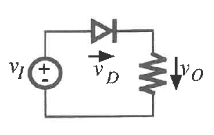
\includegraphics[width = 0.4\linewidth]{img/2/ret-meia-onda.png}
    \caption{retificador de meia onda com díodo ideal}
    \label{fig:ret-meia-onda}
\end{figure}

\noindent Supondo que a tensão no díodo, quando este conduz, não é desprezável,
utilizamos a aproximação linear por troços, nomeadamente o modelo de resistência incremental:

\begin{itemize}[leftmargin=*]
    \item Se $v_I < V_{D0}$, $v_D < 0$ e consequentemente $i_D = 0$. Díodo ideal como circuito aberto.
    \item Se $v_I > V_{D0}$, $v_D = 0$ e consequentemente $i_D > 0$. Díodo ideal equivalente a um curto circuito. Operando sobre a malha do circuito $v_o = \frac{R}{R + R_D}(v_I - V_{D0})$. Se $R_D \ll R$ fica a aproximação $v_O \simeq v_I - V_{D0}$.
\end{itemize}

\noindent No caso de $v_I$ ser uma sinusoide simplesmente retificada, tem interesse determinar o seu valor médio:
$$
    \boxed{(v_O)_{\textit{avg}} = \frac{1}{T} \int_{0}^{T} v_O(t) \, dt = \dfrac{V_m}{\pi}}
$$
\begin{mdframed}
\begin{itemize}[leftmargin=*, nolistsep]
    \item \textbf{\underline{Nota:} Dimensionamento de um díodo}
    \begin{itemize}[leftmargin=*]
    \item Dois parâmetros importantes a especificar:
        \begin{enumerate}
        \item \textbf{Capacidade de manuseio da corrente}: determinada pela maior corrente que se espera que o díodo conduza.
        \item \textbf{Tensão inversa máxima}: o díodo deve ser capaz de suportar este valor sem ocorrer disrupção (\textit{breakdown}); determinado pela maior tensão inversa esperada no díodo.
        \end{enumerate}
    \end{itemize}
\end{itemize}
\end{mdframed}

\noindent A \textbf{capacidade de manuseio da corrente} é calculada com o díodo em \textbf{curto circuito}:
$$
    \boxed{(i_D)_\textit{max} = V_m/R}
$$
\noindent A \textbf{tensão inversa máxima} é calculada com o díodo em \textbf{circuito aberto}, para o circuito em questão é dada por:
$$
    \boxed{(-v_D)_\textit{max} = V_m}
$$

\vspace{-1 em}
\begin{figure}[H]
    \centering
    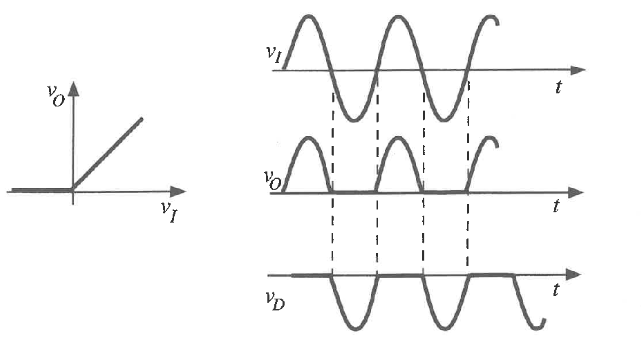
\includegraphics[width = 0.8\linewidth]{img/2/ret-curve.png}
    \caption{Curva da característica $v_O(v_I)$ e respetivo output}
    \label{fig:ret-curve}
\end{figure}

\begin{quote}
    ``Um rectificador transforma uma tensão \textbf{alternada} (com valores positivos e negativos) numa tensão \textbf{unidireccional}''\cite{medeiros:ICEE}
\end{quote}

\noindent Uma das aplicações dos retificadores de meia onda verifica-se na \textbf{desmodulação de amplitude}\footnotemark[3]. Um \textbf{detetor de pico/envolvente} pode ser implementado ao adicionar um \underline{condensador em paralelo} com a resistência de saída.

\footnotetext[3]{``Para tal, é necessário que a constante de tempo $RC$ seja muito maior que o período da sinusoide, para que o condensador não descarregue significativamente entre uma alternância e a seguinte. Por outro lado, é necessário que $RC$ seja menor que o período mínimo do sinal modulante para que $v_O$, possa acompanhar as variações da amplitude da sinusoide.''\cite{medeiros:ICEE}}

Outra aplicação significativa do retificador \underline{com condensador} é como \textbf{conversor corrente alternada/corrente contínua} (AC/DC), em \textbf{fontes de alimentação} (\textit{power supplies}).

\vspace{0.9 em}
\noindent Na realidade, nas aplicações com condensadores, a tensão de saída apresenta uma componente variável (induzida pela carga/descarga do condensador) designada por \textbf{tremor} ou \textbf{ondulação} (\textit{ripple}).

\begin{quote}
    ``Pode fazer-se uma \underline{estimativa da amplitude do tremor}, $\Delta v_O$. A carga perdida pelo condensador durante a maior parte do período,
    $$
        \Delta Q \approx I\, \Delta t = \frac{V_m}{R}\, T
    $$
    é igual a carga reposta no condensador quando o díodo conduz, durante um breve intervalo de tempo, na vizinhança do máximo de $v_I(t)$
    $$
        \Delta Q \approx C\, \Delta v_O
    $$
    Resulta que o tremor, em valor relativo, é
    $$
        \frac{\Delta v_O}{V_m} \approx \frac{T}{RC}
    $$
    Em vez de um condensador, podem usar-se filtros LC para reduzir o tremor.''\cite{medeiros:ICEE}
\end{quote}

%//==============================--@--==============================//%
\subsubsection[2.2.1 Retificadores de onda completa]{$\pmb{\rightarrow}$ Retificadores de onda completa}

\begin{quote}
    ``The full-wave rectifier utilizes both halves of the input sinusoid. To provide a unipolar output,
    it \underline{inverts the negative halves} of the wave.''\cite{sedra-smith:microelectronic-circuits}
\end{quote}

\begin{figure}[H]
    \centering
    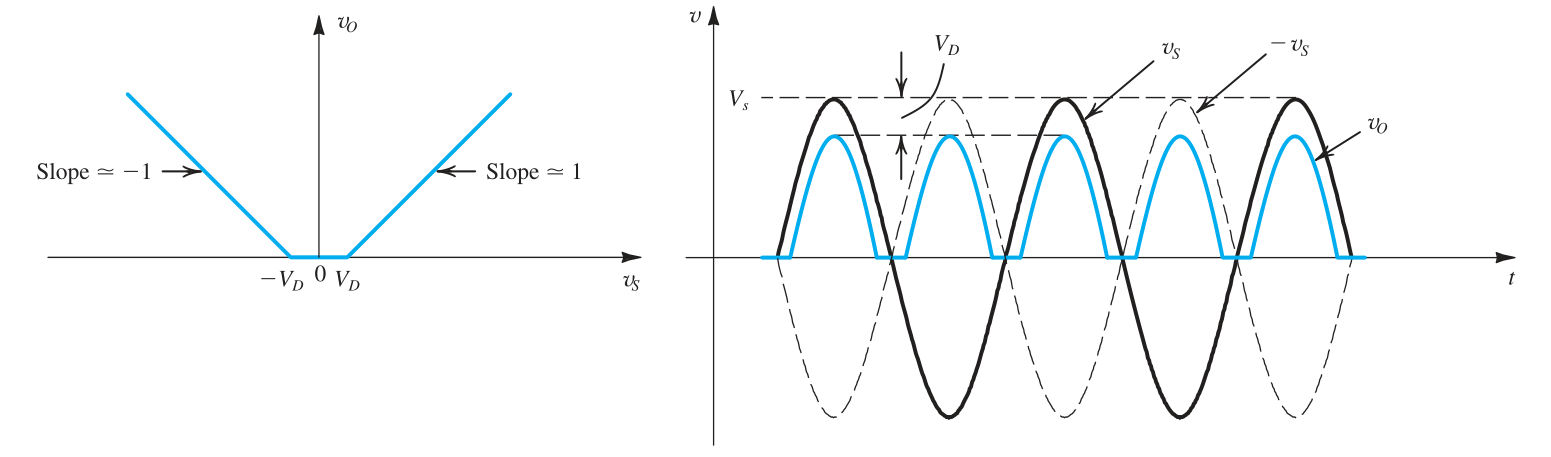
\includegraphics[width=1\linewidth]{img/2/exemplo-full-wave-rectifier.png}
    \caption{``(left) transfer characteristic assuming a constant-voltage-drop model for the diodes; (right) input and output waveforms.''\cite{sedra-smith:microelectronic-circuits}}
    \label{fig:exemplo-full-wave-rectifier}
\end{figure}

%//==============================--@--==============================//%
\paragraph[2.2.1.1 Implementação com um transformador]{$\pmb{\star}$ Implementação com um transformador}\mbox{}

\begin{figure}[H]
    \centering
    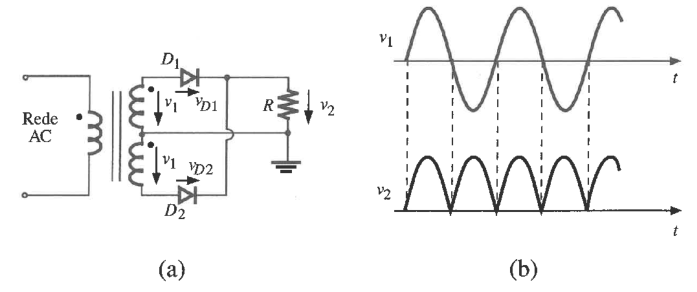
\includegraphics[width = 0.8\linewidth]{img/2/onda-completa-transformador.png}
    \caption{``Rectificador de onda completa com transformador com tomada no ponto médio do secundário.''\cite{medeiros:ICEE}}
    \label{fig:onda-completa-transformador}
\end{figure}

\noindent A ação do retificador de onda completa pode ser descrita da seguinte forma:
\begin{itemize}[leftmargin=*]
    \item Se $v_I < V_{D0}$, $v_{D1} < 0$ e $v_{D2} > 0$, D$_1$ está cortado e D$_2$ conduz. $v_2 = -v_1 - v_D \simeq - v_1$
    \item Se $v_I > V_{D0}$, $v_{D1} > 0$ e $v_{D2} < 0$, D$_2$ está cortado e D$_1$ conduz. $v_2 = v_1 + v_D \simeq  v_1$
    \item Logo $v_2 \simeq |v_1|$
\end{itemize}

\noindent No caso de $v_I$ ser uma sinusoide simplesmente retificada, podemos calcular novamente o seu o seu valor médio:
$$
    \boxed{(v_2)_{\textit{avg}} = \frac{1}{T} \int_{0}^{T} v_O(t) \, dt = \dfrac{2V_m}{\pi}}
$$

\noindent A \textbf{tensão inversa máxima} é calculada com o díodo 1 ou 2 em \textbf{circuito aberto}. Supondo $v_I > V_{D0}$ e o díodo 2 em aberto:
$$
    v_{D2} = -V_I - V_2\; \pmb{\longrightarrow}\; (-v_D)_{\text{máx}} = V_I + V_2
$$
\noindent $V_2$ é máximo para $V_I - V_{D1}$, logo:
$$
    \boxed{(-v_D)_{\text{max}} = 2V_m - V_{D1}}
$$

%//==============================--@--==============================//%
\clearpage
\paragraph[2.2.1.2 Implementação em ponte de Graetz]{$\pmb{\star}$ Implementação em ponte de Graetz (\textit{Bridge Rectifier})}\mbox{}

\begin{quote}
    ``An alternative implementation of the full-wave rectifier is the bridge rectifier. This circuit, is known as the bridge rectifier because of the similarity of its configuration to that of the Wheatstone bridge, does not require a center-tapped transformer, a distinct advantage over the full-wave rectifier circuit"\cite{sedra-smith:microelectronic-circuits}
\end{quote}

\begin{figure}[H]
    \centering
    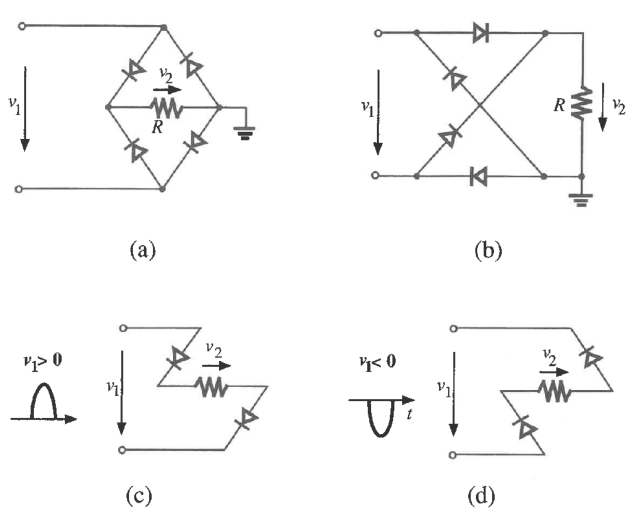
\includegraphics[width = 0.65\linewidth]{img/2/ponte-graetz.png}
    \caption{``Rectificador em ponte de Graetz.''\cite{medeiros:ICEE}}
    \label{fig:ponte-graetz}
\end{figure}

\begin{itemize}
    \item Nas alternâncias positivas de $v_i$, apenas conduzem dois dos díodos, como se indica na \hyperref[fig:ponte-graetz]{Fig. 12 (c)}, obtendo-se:
    $$
        v_2 = v_1 - 2V_D \simeq v_1
    $$
    \item Nas alternâncias negativas de $v_i$, conduzem os díodos contrários, como se indica na \hyperref[fig:ponte-graetz]{Fig. 12 (d)}, obtendo-se:
    $$
        v_2 = - v_1 - 2V_D \simeq  - v_1
    $$
    \item Logo:
    $$
        v_2 \simeq |v_1|
    $$
\end{itemize}

\noindent A \textbf{tensão inversa máxima} é dada por:
$$
    v_{D2} = -V_D - V_2\; \pmb{\longrightarrow}\; (-v_D)_{\text{máx}} = V_D + V_2
$$
\noindent $V_2$ é máximo para $V_m - 2V_{D}$, logo:
$$
    \boxed{(-v_D)_{\text{max}} = V_m - V_{D}}
$$

\noindent Comparando o rectificador em ponte com o circuito anterior, pode concluir-se que o circuito em ponte emprega quatro díodos, em vez de dois, mas tem as seguintes vantagens:

\begin{itemize}
    \item  O transformador é mais simples, uma vez que o secundário não tem tomada central e, para as mesmas tensões, tem metade do número de espiras;
    \item \underline{Tensão inversa máxima} nos díodos é aproximadamente \underline{metade}.
\end{itemize}

%//==============================--@--==============================//%